\documentclass[11pt,compress,t,notes=noshow, xcolor=table]{beamer}


% graphicx and color are loaded via lmu-lecture.sty
% maxwidth is the original width if it is less than linewidth
% otherwise use linewidth (to make sure the graphics do not exceed the margin)
% TODO: Remove once cleared to be superfluous
% \makeatletter
% \def\maxwidth{ %
%   \ifdim\Gin@nat@width>\linewidth
%     \linewidth
%   \else
%     \Gin@nat@width
%   \fi
% }
% \makeatother

% ---------------------------------%
% latex-math dependencies, do not remove:
% - mathtools
% - bm
% - siunitx
% - dsfont
% - xspace
% ---------------------------------%

%--------------------------------------------------------%
%       Language, encoding, typography
%--------------------------------------------------------%

\usepackage[english]{babel}
\usepackage[utf8]{inputenc} % Enables inputting UTF-8 symbols
% Standard AMS suite (loaded via lmu-lecture.sty)

% Font for double-stroke / blackboard letters for sets of numbers (N, R, ...)
% Distribution name is "doublestroke"
% According to https://mirror.physik.tu-berlin.de/pub/CTAN/fonts/doublestroke/dsdoc.pdf
% the "bbm" package does a similar thing and may be superfluous.
% Required for latex-math
\usepackage{dsfont}

% bbm – "Blackboard-style" cm fonts (https://www.ctan.org/pkg/bbm)
% Used to be in common.tex, loaded directly after this file
% Maybe superfluous given dsfont is loaded
% TODO: Check if really unused?
% \usepackage{bbm}

% bm – Access bold symbols in maths mode - https://ctan.org/pkg/bm
% Required for latex-math, preferred over \boldsymbol
% https://tex.stackexchange.com/questions/3238/bm-package-versus-boldsymbol
\usepackage{bm}

% pifont – Access to PostScript standard Symbol and Dingbats fonts
% Used for \newcommand{\xmark}{\ding{55}, which is never used
% aside from lecture_advml/attic/xx-automl/slides.Rnw
% \usepackage{pifont}

% Quotes (inline and display), provdes \enquote
% https://ctan.org/pkg/csquotes
\usepackage{csquotes}

% Adds arg to enumerate env, technically superseded by enumitem according
% to https://ctan.org/pkg/enumerate
% Replace with https://ctan.org/pkg/enumitem ?
% Even better: enumitem is not really compatible with beamer and breaks all sorts of things
% particularly the enumerate environment. The enumerate package also just isn't required
% from what I can tell so... don't re-add it I guess?
% \usepackage{enumerate}

% Line spacing - provides \singlespacing \doublespacing \onehalfspacing
% https://ctan.org/pkg/setspace
% \usepackage{setspace}

% mathtools – Mathematical tools to use with amsmath
% https://ctan.org/pkg/mathtools?lang=en
% latex-math dependency according to latex-math repo
\usepackage{mathtools}

% Maybe not great to use this https://tex.stackexchange.com/a/197/19093
% Use align instead -- TODO: Global search & replace to check, eqnarray is used a lot
% $ rg -f -u "\begin{eqnarray" -l | grep -v attic | awk -F '/' '{print $1}' | sort | uniq -c
%   13 lecture_advml
%   14 lecture_i2ml
%    2 lecture_iml
%   27 lecture_optimization
%   45 lecture_sl
\usepackage{eqnarray}
% For shaded regions / boxes
% Used sometimes in optim
% https://www.ctan.org/pkg/framed
\usepackage{framed}

%--------------------------------------------------------%
%       Cite button (version 2024-05)
%--------------------------------------------------------%

% Superseded by style/ref-buttons.sty, kept just in case these don't work out somehow.

% Note this requires biber to be in $PATH when running,
% telltale error in log would be e.g. Package biblatex Info: ... file 'authoryear.dbx' not found
% aside from obvious "biber: command not found" or similar.
% Tried moving this to lmu-lecture.sty but had issues I didn't quite understood,
% so it's here for now.

\usepackage{hyperref}

% Only try adding a references file if it exists, otherwise
% this would compile error when references.bib is not found
% NOTE: Bibliography packages (usebib, biblatex) are now loaded by ref-buttons.sty when needed
% This keeps all bibliography-related setup in one place

% Legacy \citelink command removed - superseded by ref-buttons.sty

%--------------------------------------------------------%
%       Displaying code and algorithms
%--------------------------------------------------------%

% Reimplements verbatim environments: https://ctan.org/pkg/verbatim
% verbatim used sed at least once in
% supervised-classification/slides-classification-tasks.tex
% Removed since code should not be put on slides anyway
% \usepackage{verbatim}

% Both used together for algorithm typesetting, see also overleaf: https://www.overleaf.com/learn/latex/Algorithms
% algorithmic env is also used, but part of the bundle:
%   "algpseudocode is part of the algorithmicx bundle, it gives you an improved version of algorithmic besides providing some other features"
% According to https://tex.stackexchange.com/questions/229355/algorithm-algorithmic-algorithmicx-algorithm2e-algpseudocode-confused
\usepackage{algorithm}
\usepackage{algpseudocode}

%--------------------------------------------------------%
%       Tables
%--------------------------------------------------------%

% multi-row table cells: https://www.namsu.de/Extra/pakete/Multirow.html
% Provides \multirow
% Used e.g. in evaluation/slides-evaluation-measures-classification.tex
\usepackage{multirow}

% colortbl: https://ctan.org/pkg/colortbl
% "The package allows rows and columns to be coloured, and even individual cells." well.
% Provides \columncolor and \rowcolor
% \rowcolor is used multiple times, e.g. in knn/slides-knn.tex
\usepackage{colortbl}

% long/multi-page tables: https://texdoc.org/serve/longtable.pdf/0
% Not used in slides
% \usepackage{longtable}

% pretty table env: https://ctan.org/pkg/booktabs
% Is used
% Defines \toprule
\usepackage{booktabs}

%--------------------------------------------------------%
%       Figures: Creating, placing, verbing
%--------------------------------------------------------%

% wrapfig - Wrapping text around figures https://de.overleaf.com/learn/latex/Wrapping_text_around_figures
% Provides wrapfigure environment -used in lecture_optimization
\usepackage{wrapfig}

% Sub figures in figures and tables
% https://ctan.org/pkg/subfig -- supersedes subfigure package
% Provides \subfigure
% \subfigure not used in slides but slides-tuning-practical.pdf errors without this pkg, error due to \captionsetup undefined
\usepackage{subfig}

% Actually it's pronounced PGF https://en.wikibooks.org/wiki/LaTeX/PGF/TikZ
\usepackage{tikz}

% No idea what/why these settings are what they are but I assume they're there on purpose
\usetikzlibrary{shapes,arrows,automata,positioning,calc,chains,trees, shadows}
\tikzset{
  %Define standard arrow tip
  >=stealth',
  %Define style for boxes
  punkt/.style={
    rectangle,
    rounded corners,
    draw=black, very thick,
    text width=6.5em,
    minimum height=2em,
    text centered},
  % Define arrow style
  pil/.style={
    ->,
    thick,
    shorten <=2pt,
    shorten >=2pt,}
}

%--------------------------------------------------------%
%       Beamer setup and custom macros & environments
%--------------------------------------------------------%

% Main sty file for beamer setup (layout, style, lecture page numbering, etc.)
% For long-term maintenance, this may me refactored into a more modular set of .sty files
\usepackage{../../style/lmu-lecture}
% Custom itemize wrappers, itemizeS, itemizeL, etc
\usepackage{../../style/customitemize}
% Custom framei environment, uses custom itemize!
\usepackage{../../style/framei}
% Custom frame2 environment, allows specifying font size for all content
\usepackage{../../style/frame2}
% Column layout macros
\usepackage{../../style/splitV}
% \image and derivatives
\usepackage{../../style/image}
% New generation of reference button macros
\usepackage{../../style/ref-buttons}

% Used regularly
\let\code=\texttt

% Not sure what/why this does
\setkeys{Gin}{width=0.9\textwidth}

% -- knitr leftovers --
% These may be used by knitr/R Markdown workflows in other lectures
\makeatletter
\def\maxwidth{ %
  \ifdim\Gin@nat@width>\linewidth
    \linewidth
  \else
    \Gin@nat@width
  \fi
}
\makeatother

% Define colors for syntax highlighting (may be used by knitr)
\definecolor{fgcolor}{rgb}{0.345, 0.345, 0.345}
\definecolor{shadecolor}{rgb}{.97, .97, .97}

% knitr code output environment
\newenvironment{knitrout}{}{}


% Can't find a reason why common.tex is not just part of this file?
% This file is included in slides and exercises

% Rarely used fontstyle for R packages, used only in 
% - forests/slides-forests-benchmark.tex
% - exercises/single-exercises/methods_l_1.Rnw
% - slides/cart/attic/slides_extra_trees.Rnw
\newcommand{\pkg}[1]{{\fontseries{b}\selectfont #1}}

% Spacing helpers, used often (mostly in exercises for \dlz)
\newcommand{\lz}{\vspace{0.5cm}} % vertical space (used often in slides)
\newcommand{\dlz}{\vspace{1cm}}  % double vertical space (used often in exercises, never in slides)
\newcommand{\oneliner}[1] % Oneliner for important statements, used e.g. in iml, algods
{\begin{block}{}\begin{center}\begin{Large}#1\end{Large}\end{center}\end{block}}

% Don't know if this is used or needed, remove?
% textcolor that works in mathmode
% https://tex.stackexchange.com/a/261480
% Used e.g. in forests/slides-forests-bagging.tex
% [...] \textcolor{blue}{\tfrac{1}{M}\sum^M_{m} [...]
% \makeatletter
% \renewcommand*{\@textcolor}[3]{%
%   \protect\leavevmode
%   \begingroup
%     \color#1{#2}#3%
%   \endgroup
% }
% \makeatother


% math spaces
\ifdefined\N                                                                
\renewcommand{\N}{\mathds{N}} % N, naturals
\else \newcommand{\N}{\mathds{N}} \fi 
\newcommand{\Z}{\mathds{Z}} % Z, integers
\newcommand{\Q}{\mathds{Q}} % Q, rationals
\newcommand{\R}{\mathds{R}} % R, reals
\ifdefined\C 
  \renewcommand{\C}{\mathds{C}} % C, complex
\else \newcommand{\C}{\mathds{C}} \fi
\newcommand{\continuous}{\mathcal{C}} % C, space of continuous functions
\newcommand{\M}{\mathcal{M}} % machine numbers
\newcommand{\epsm}{\epsilon_m} % maximum error

% counting / finite sets
\newcommand{\setzo}{\{0, 1\}} % set 0, 1
\newcommand{\setmp}{\{-1, +1\}} % set -1, 1
\newcommand{\unitint}{[0, 1]} % unit interval

% basic math stuff
\newcommand{\xt}{\tilde x} % x tilde
\newcommand{\argmax}{\operatorname{arg\,max}} % argmax
\newcommand{\argmin}{\operatorname{arg\,min}} % argmin
\newcommand{\argopt}{\operatorname{arg\,opt}} % argopt
\newcommand{\argminlim}{\mathop{\mathrm{arg\,min}}\limits} % argmax with limits
\newcommand{\argmaxlim}{\mathop{\mathrm{arg\,max}}\limits} % argmin with limits  
\newcommand{\argoptlim}{\mathop{\mathrm{arg\,opt}}\limits} % argmin with limits  
\newcommand{\sign}{\operatorname{sign}} % sign, signum
\newcommand{\I}{\mathbb{I}} % I, indicator
\newcommand{\order}{\mathcal{O}} % O, order
\newcommand{\pd}[2]{\frac{\partial{#1}}{\partial #2}} % partial derivative
\newcommand{\floorlr}[1]{\left\lfloor #1 \right\rfloor} % floor
\newcommand{\ceillr}[1]{\left\lceil #1 \right\rceil} % ceiling

% sums and products
\newcommand{\sumin}{\sum\limits_{i=1}^n} % summation from i=1 to n
\newcommand{\sumim}{\sum\limits_{i=1}^m} % summation from i=1 to m
\newcommand{\sumjn}{\sum\limits_{j=1}^n} % summation from j=1 to p
\newcommand{\sumjp}{\sum\limits_{j=1}^p} % summation from j=1 to p
\newcommand{\sumik}{\sum\limits_{i=1}^k} % summation from i=1 to k
\newcommand{\sumkg}{\sum\limits_{k=1}^g} % summation from k=1 to g
\newcommand{\sumjg}{\sum\limits_{j=1}^g} % summation from j=1 to g
\newcommand{\meanin}{\frac{1}{n} \sum\limits_{i=1}^n} % mean from i=1 to n
\newcommand{\meankg}{\frac{1}{g} \sum\limits_{k=1}^g} % mean from k=1 to g
\newcommand{\prodin}{\prod\limits_{i=1}^n} % product from i=1 to n
\newcommand{\prodkg}{\prod\limits_{k=1}^g} % product from k=1 to g
\newcommand{\prodjp}{\prod\limits_{j=1}^p} % product from j=1 to p

% linear algebra
\newcommand{\one}{\boldsymbol{1}} % 1, unitvector
\newcommand{\zero}{\mathbf{0}} % 0-vector
\newcommand{\id}{\boldsymbol{I}} % I, identity
\newcommand{\diag}{\operatorname{diag}} % diag, diagonal
\newcommand{\trace}{\operatorname{tr}} % tr, trace
\newcommand{\spn}{\operatorname{span}} % span
\newcommand{\scp}[2]{\left\langle #1, #2 \right\rangle} % <.,.>, scalarproduct
\newcommand{\mat}[1]{\begin{pmatrix} #1 \end{pmatrix}} % short pmatrix command
\newcommand{\Amat}{\mathbf{A}} % matrix A
\newcommand{\Deltab}{\mathbf{\Delta}} % error term for vectors

% basic probability + stats
\renewcommand{\P}{\mathds{P}} % P, probability
\newcommand{\E}{\mathds{E}} % E, expectation
\newcommand{\var}{\mathsf{Var}} % Var, variance
\newcommand{\cov}{\mathsf{Cov}} % Cov, covariance
\newcommand{\corr}{\mathsf{Corr}} % Corr, correlation
\newcommand{\normal}{\mathcal{N}} % N of the normal distribution
\newcommand{\iid}{\overset{i.i.d}{\sim}} % dist with i.i.d superscript
\newcommand{\distas}[1]{\overset{#1}{\sim}} % ... is distributed as ...
% machine learning
\newcommand{\Xspace}{\mathcal{X}} % X, input space
\newcommand{\Yspace}{\mathcal{Y}} % Y, output space
\newcommand{\Zspace}{\mathcal{Z}} % Z, space of sampled datapoints
\newcommand{\nset}{\{1, \ldots, n\}} % set from 1 to n
\newcommand{\pset}{\{1, \ldots, p\}} % set from 1 to p
\newcommand{\gset}{\{1, \ldots, g\}} % set from 1 to g
\newcommand{\Pxy}{\mathbb{P}_{xy}} % P_xy
\newcommand{\Exy}{\mathbb{E}_{xy}} % E_xy: Expectation over random variables xy
\newcommand{\xv}{\mathbf{x}} % vector x (bold)
\newcommand{\xtil}{\tilde{\mathbf{x}}} % vector x-tilde (bold)
\newcommand{\yv}{\mathbf{y}} % vector y (bold)
\newcommand{\xy}{(\xv, y)} % observation (x, y)
\newcommand{\xvec}{\left(x_1, \ldots, x_p\right)^\top} % (x1, ..., xp)
\newcommand{\Xmat}{\mathbf{X}} % Design matrix
\newcommand{\allDatasets}{\mathds{D}} % The set of all datasets
\newcommand{\allDatasetsn}{\mathds{D}_n}  % The set of all datasets of size n
\newcommand{\D}{\mathcal{D}} % D, data
\newcommand{\Dn}{\D_n} % D_n, data of size n
\newcommand{\Dtrain}{\mathcal{D}_{\text{train}}} % D_train, training set
\newcommand{\Dtest}{\mathcal{D}_{\text{test}}} % D_test, test set
\newcommand{\xyi}[1][i]{\left(\xv^{(#1)}, y^{(#1)}\right)} % (x^i, y^i), i-th observation
\newcommand{\Dset}{\left( \xyi[1], \ldots, \xyi[n]\right)} % {(x1,y1)), ..., (xn,yn)}, data
\newcommand{\defAllDatasetsn}{(\Xspace \times \Yspace)^n} % Def. of the set of all datasets of size n
\newcommand{\defAllDatasets}{\bigcup_{n \in \N}(\Xspace \times \Yspace)^n} % Def. of the set of all datasets
\newcommand{\xdat}{\left\{ \xv^{(1)}, \ldots, \xv^{(n)}\right\}} % {x1, ..., xn}, input data
\newcommand{\ydat}{\left\{ \yv^{(1)}, \ldots, \yv^{(n)}\right\}} % {y1, ..., yn}, input data
\newcommand{\yvec}{\left(y^{(1)}, \hdots, y^{(n)}\right)^\top} % (y1, ..., yn), vector of outcomes
\newcommand{\greekxi}{\xi} % Greek letter xi
\renewcommand{\xi}[1][i]{\xv^{(#1)}} % x^i, i-th observed value of x
\newcommand{\yi}[1][i]{y^{(#1)}} % y^i, i-th observed value of y
\newcommand{\xivec}{\left(x^{(i)}_1, \ldots, x^{(i)}_p\right)^\top} % (x1^i, ..., xp^i), i-th observation vector
\newcommand{\xj}{\xv_j} % x_j, j-th feature
\newcommand{\xjvec}{\left(x^{(1)}_j, \ldots, x^{(n)}_j\right)^\top} % (x^1_j, ..., x^n_j), j-th feature vector
\newcommand{\phiv}{\mathbf{\phi}} % Basis transformation function phi
\newcommand{\phixi}{\mathbf{\phi}^{(i)}} % Basis transformation of xi: phi^i := phi(xi)

%%%%%% ml - models general
\newcommand{\lamv}{\bm{\lambda}} % lambda vector, hyperconfiguration vector
\newcommand{\Lam}{\Lambda}	 % Lambda, space of all hpos
% Inducer / Inducing algorithm
\newcommand{\preimageInducer}{\left(\defAllDatasets\right)\times\Lam} % Set of all datasets times the hyperparameter space
\newcommand{\preimageInducerShort}{\allDatasets\times\Lam} % Set of all datasets times the hyperparameter space
% Inducer / Inducing algorithm
\newcommand{\ind}{\mathcal{I}} % Inducer, inducing algorithm, learning algorithm

% continuous prediction function f
\newcommand{\ftrue}{f_{\text{true}}}  % True underlying function (if a statistical model is assumed)
\newcommand{\ftruex}{\ftrue(\xv)} % True underlying function (if a statistical model is assumed)
\newcommand{\fx}{f(\xv)} % f(x), continuous prediction function
\newcommand{\fdomains}{f: \Xspace \rightarrow \R^g} % f with domain and co-domain
\newcommand{\Hspace}{\mathcal{H}} % hypothesis space where f is from
\newcommand{\Hall}{\mathcal{H}_{\text{all}}} % unrestricted hypothesis space
\newcommand{\fbayes}{f^{\ast}} % Bayes-optimal model
\newcommand{\fxbayes}{f^{\ast}(\xv)} % Bayes-optimal model
\newcommand{\fkx}[1][k]{f_{#1}(\xv)} % f_j(x), discriminant component function
\newcommand{\fhspace}{\hat f_{\Hspace}} % fhat_H
\newcommand{\fh}{\hat{f}} % f hat, estimated prediction function
\newcommand{\fxh}{\fh(\xv)} % fhat(x)
\newcommand{\fxt}{f(\xv ~|~ \thetav)} % f(x | theta)
\newcommand{\fxi}{f\left(\xv^{(i)}\right)} % f(x^(i))
\newcommand{\fxih}{\hat{f}\left(\xv^{(i)}\right)} % f(x^(i))
\newcommand{\fxit}{f\big(\xv^{(i)} ~|~ \thetav\big)} % f(x^(i) | theta)
\newcommand{\fhD}{\fh_{\D}} % fhat_D, estimate of f based on D
\newcommand{\fhDtrain}{\fh_{\Dtrain}} % fhat_Dtrain, estimate of f based on D
\newcommand{\fhDnlam}{\fh_{\Dn, \lamv}} %model learned on Dn with hp lambda
\newcommand{\fhDlam}{\fh_{\D, \lamv}} %model learned on D with hp lambda
\newcommand{\fhDnlams}{\fh_{\Dn, \lamv^\ast}} %model learned on Dn with optimal hp lambda
\newcommand{\fhDlams}{\fh_{\D, \lamv^\ast}} %model learned on D with optimal hp lambda

% discrete prediction function h
\newcommand{\hx}{h(\xv)} % h(x), discrete prediction function
\newcommand{\hh}{\hat{h}} % h hat
\newcommand{\hxh}{\hat{h}(\xv)} % hhat(x)
\newcommand{\hxt}{h(\xv | \thetav)} % h(x | theta)
\newcommand{\hxi}{h\left(\xi\right)} % h(x^(i))
\newcommand{\hxit}{h\left(\xi ~|~ \thetav\right)} % h(x^(i) | theta)
\newcommand{\hbayes}{h^{\ast}} % Bayes-optimal classification model
\newcommand{\hxbayes}{h^{\ast}(\xv)} % Bayes-optimal classification model

% yhat
\newcommand{\yh}{\hat{y}} % yhat for prediction of target
\newcommand{\yih}{\hat{y}^{(i)}} % yhat^(i) for prediction of ith targiet
\newcommand{\resi}{\yi- \yih}

% theta
\newcommand{\thetah}{\hat{\theta}} % theta hat
\newcommand{\thetav}{\bm{\theta}} % theta vector
\newcommand{\thetavh}{\bm{\hat\theta}} % theta vector hat
\newcommand{\thetat}[1][t]{\thetav^{[#1]}} % theta^[t] in optimization
\newcommand{\thetatn}[1][t]{\thetav^{[#1 +1]}} % theta^[t+1] in optimization
\newcommand{\thetahDnlam}{\thetavh_{\Dn, \lamv}} %theta learned on Dn with hp lambda
\newcommand{\thetahDlam}{\thetavh_{\D, \lamv}} %theta learned on D with hp lambda
\newcommand{\mint}{\min_{\thetav \in \Theta}} % min problem theta
\newcommand{\argmint}{\argmin_{\thetav \in \Theta}} % argmin theta

% densities + probabilities
% pdf of x
\newcommand{\pdf}{p} % p
\newcommand{\pdfx}{p(\xv)} % p(x)
\newcommand{\pixt}{\pi(\xv~|~ \thetav)} % pi(x|theta), pdf of x given theta
\newcommand{\pixit}[1][i]{\pi\left(\xi[#1] ~|~ \thetav\right)} % pi(x^i|theta), pdf of x given theta
\newcommand{\pixii}[1][i]{\pi\left(\xi[#1]\right)} % pi(x^i), pdf of i-th x

% pdf of (x, y)
\newcommand{\pdfxy}{p(\xv,y)} % p(x, y)
\newcommand{\pdfxyt}{p(\xv, y ~|~ \thetav)} % p(x, y | theta)
\newcommand{\pdfxyit}{p\left(\xi, \yi ~|~ \thetav\right)} % p(x^(i), y^(i) | theta)

% pdf of x given y
\newcommand{\pdfxyk}[1][k]{p(\xv | y= #1)} % p(x | y = k)
\newcommand{\lpdfxyk}[1][k]{\log p(\xv | y= #1)} % log p(x | y = k)
\newcommand{\pdfxiyk}[1][k]{p\left(\xi | y= #1 \right)} % p(x^i | y = k)

% prior probabilities
\newcommand{\pik}[1][k]{\pi_{#1}} % pi_k, prior
\newcommand{\pih}{\hat{\pi}} % pi hat, estimated prior (binary classification)
\newcommand{\pikh}[1][k]{\hat{\pi}_{#1}} % pi_k hat, estimated prior
\newcommand{\lpik}[1][k]{\log \pi_{#1}} % log pi_k, log of the prior
\newcommand{\pit}{\pi(\thetav)} % Prior probability of parameter theta

% posterior probabilities
\newcommand{\post}{\P(y = 1 ~|~ \xv)} % P(y = 1 | x), post. prob for y=1
\newcommand{\postk}[1][k]{\P(y = #1 ~|~ \xv)} % P(y = k | y), post. prob for y=k
\newcommand{\pidomains}{\pi: \Xspace \rightarrow \unitint} % pi with domain and co-domain
\newcommand{\pibayes}{\pi^{\ast}} % Bayes-optimal classification model
\newcommand{\pixbayes}{\pi^{\ast}(\xv)} % Bayes-optimal classification model
\newcommand{\piastxtil}{\pi^{\ast}(\xtil)} % Bayes-optimal classification model
\newcommand{\piastkxtil}{\pi^{\ast}_k(\xtil)} % Bayes-optimal classification model for k-th class
\newcommand{\pix}{\pi(\xv)} % pi(x), P(y = 1 | x)
\newcommand{\piv}{\bm{\pi}} % pi, bold, as vector
\newcommand{\pikx}[1][k]{\pi_{#1}(\xv)} % pi_k(x), P(y = k | x)
\newcommand{\pikxt}[1][k]{\pi_{#1}(\xv ~|~ \thetav)} % pi_k(x | theta), P(y = k | x, theta)
\newcommand{\pixh}{\hat \pi(\xv)} % pi(x) hat, P(y = 1 | x) hat
\newcommand{\pikxh}[1][k]{\hat \pi_{#1}(\xv)} % pi_k(x) hat, P(y = k | x) hat
\newcommand{\pixih}{\hat \pi(\xi)} % pi(x^(i)) with hat
\newcommand{\pikxih}[1][k]{\hat \pi_{#1}(\xi)} % pi_k(x^(i)) with hat
\newcommand{\pdfygxt}{p(y ~|~\xv, \thetav)} % p(y | x, theta)
\newcommand{\pdfyigxit}{p\left(\yi ~|~\xi, \thetav\right)} % p(y^i |x^i, theta)
\newcommand{\lpdfygxt}{\log \pdfygxt } % log p(y | x, theta)
\newcommand{\lpdfyigxit}{\log \pdfyigxit} % log p(y^i |x^i, theta)

% probabilistic
\newcommand{\bayesrulek}[1][k]{\frac{\P(\xv | y= #1) \P(y= #1)}{\P(\xv)}} % Bayes rule
\newcommand{\muv}{\bm{\mu}} % expectation vector of Gaussian
\newcommand{\muk}[1][k]{\bm{\mu_{#1}}} % mean vector of class-k Gaussian (discr analysis)
\newcommand{\mukh}[1][k]{\bm{\hat{\mu}_{#1}}} % estimated mean vector of class-k Gaussian (discr analysis)

% residual and margin
\newcommand{\rx}{r(\xv)} % residual 
\newcommand{\eps}{\epsilon} % residual, stochastic
\newcommand{\epsv}{\bm{\epsilon}} % residual, stochastic, as vector
\newcommand{\epsi}{\epsilon^{(i)}} % epsilon^i, residual, stochastic
\newcommand{\epsh}{\hat{\epsilon}} % residual, estimated
\newcommand{\epsvh}{\hat{\epsv}} % residual, estimated, vector
\newcommand{\yf}{y \fx} % y f(x), margin
\newcommand{\yfi}{\yi \fxi} % y^i f(x^i), margin
\newcommand{\Sigmah}{\hat \Sigma} % estimated covariance matrix
\newcommand{\Sigmahj}{\hat \Sigma_j} % estimated covariance matrix for the j-th class
\newcommand{\nux}{\nu(\xv)} % nu(x) = y * f(x)

% ml - loss, risk, likelihood
\newcommand{\Lyf}{L\left(y, f\right)} % L(y, f), loss function
% \newcommand{\Lypi}{L\left(y, \pi\right)} % L(y, pi), loss function
\newcommand{\Lxy}{L\left(y, \fx\right)} % L(y, f(x)), loss function
\newcommand{\Lxyi}{L\left(\yi, \fxi\right)} % loss of observation
\newcommand{\Lxyt}{L\left(y, \fxt\right)} % loss with f parameterized
\newcommand{\Lxyit}{L\left(\yi, \fxit\right)} % loss of observation with f parameterized
\newcommand{\Lxym}{L\left(\yi, f\left(\bm{\tilde{x}}^{(i)} ~|~ \thetav\right)\right)} % loss of observation with f parameterized
\newcommand{\Lpixy}{L\left(y, \pix\right)} % loss in classification
% \newcommand{\Lpiy}{L\left(y, \pi\right)} % loss in classification
\newcommand{\Lpiv}{L\left(y, \piv\right)} % loss in classification
\newcommand{\Lpixyi}{L\left(\yi, \pixii\right)} % loss of observation in classification
\newcommand{\Lpixyt}{L\left(y, \pixt\right)} % loss with pi parameterized
\newcommand{\Lpixyit}{L\left(\yi, \pixit\right)} % loss of observation with pi parameterized
% \newcommand{\Lhy}{L\left(y, h\right)} % L(y, h), loss function on discrete classes
\newcommand{\Lhxy}{L\left(y, \hx\right)} % L(y, h(x)), loss function on discrete classes
\newcommand{\Lr}{L\left(r\right)} % L(r), loss defined on residual (reg) / margin (classif)
\newcommand{\lone}{|y - \fx|} % L1 loss
\newcommand{\ltwo}{\left(y - \fx\right)^2} % L2 loss
\newcommand{\lbernoullimp}{\ln(1 + \exp(-y \cdot \fx))} % Bernoulli loss for -1, +1 encoding
\newcommand{\lbernoullizo}{- y \cdot \fx + \log(1 + \exp(\fx))} % Bernoulli loss for 0, 1 encoding
\newcommand{\lcrossent}{- y \log \left(\pix\right) - (1 - y) \log \left(1 - \pix\right)} % cross-entropy loss
\newcommand{\lbrier}{\left(\pix - y \right)^2} % Brier score
\newcommand{\risk}{\mathcal{R}} % R, risk
\newcommand{\riskbayes}{\mathcal{R}^\ast}
\newcommand{\riskf}{\risk(f)} % R(f), risk
\newcommand{\riskdef}{\E_{y|\xv}\left(\Lxy \right)} % risk def (expected loss)
\newcommand{\riskt}{\mathcal{R}(\thetav)} % R(theta), risk
\newcommand{\riske}{\mathcal{R}_{\text{emp}}} % R_emp, empirical risk w/o factor 1 / n
\newcommand{\riskeb}{\bar{\mathcal{R}}_{\text{emp}}} % R_emp, empirical risk w/ factor 1 / n
\newcommand{\riskef}{\riske(f)} % R_emp(f)
\newcommand{\risket}{\mathcal{R}_{\text{emp}}(\thetav)} % R_emp(theta)
\newcommand{\riskr}{\mathcal{R}_{\text{reg}}} % R_reg, regularized risk
\newcommand{\riskrt}{\mathcal{R}_{\text{reg}}(\thetav)} % R_reg(theta)
\newcommand{\riskrf}{\riskr(f)} % R_reg(f)
\newcommand{\riskrth}{\hat{\mathcal{R}}_{\text{reg}}(\thetav)} % hat R_reg(theta)
\newcommand{\risketh}{\hat{\mathcal{R}}_{\text{emp}}(\thetav)} % hat R_emp(theta)
\newcommand{\LL}{\mathcal{L}} % L, likelihood
\newcommand{\LLt}{\mathcal{L}(\thetav)} % L(theta), likelihood
\newcommand{\LLtx}{\mathcal{L}(\thetav | \xv)} % L(theta|x), likelihood
\newcommand{\logl}{\ell} % l, log-likelihood
\newcommand{\loglt}{\logl(\thetav)} % l(theta), log-likelihood
\newcommand{\logltx}{\logl(\thetav | \xv)} % l(theta|x), log-likelihood
\newcommand{\errtrain}{\text{err}_{\text{train}}} % training error
\newcommand{\errtest}{\text{err}_{\text{test}}} % test error
\newcommand{\errexp}{\overline{\text{err}_{\text{test}}}} % avg training error

% lm
\newcommand{\thx}{\thetav^\top \xv} % linear model
\newcommand{\olsest}{(\Xmat^\top \Xmat)^{-1} \Xmat^\top \yv} % OLS estimator in LM



\usepackage{etoolbox}
\makeatletter
\newlength{\parboxtodim}
\patchcmd{\@iiiparbox}
  {\hsize}
  {\ifx\relax#2\else\setlength{\parboxtodim}{#2}\fi\hsize}
  {}{}
\makeatother


\setbeamersize{text margin left=0.3cm,text margin right=0.3cm}

\begin{document}

\title{Applied Machine Learning}

\titlemeta{
Performance Evaluation:
}{
Calibration Methods \& Practices
}{
figure/calibrationplot
}{
\item How to calibrate probabilities using different methods
\item Best practices for data splitting in calibration
}


\begin{frame}{Calibrating Probabilities}

\textbf{Goal}: Calibration Techniques

\begin{itemize}
  \item Calibrating probabilities involves \textbf{post-processing} predictions. % to improve their reliability.
  %Calibrating probabilities means to \textbf{post-process} the predictions.% to improve the estimates and obtain more reliable probabilities.
  %\item Two popular calibration methods are the \textbf{Platt’s scaling} (parametric) and the \textbf{isotonic regression} (non-parametric).
  %\item A well calibrated classifier should classify samples such that among these samples with a predicted probability of 0.7, approximately 70\% actually belong to the positive class.
  \item \textbf{Aim:} Ensure predicted probabilities of any event should (on average) match their observed empirical probabilities.\\
    $\Rightarrow$ Makes predictions interpretable as actual risk/probabilities.
  \item Calibration should be performed on \textbf{new data} not used for model fitting.
  \item Link function in \textbf{logistic regression} can be viewed as a calibration of predictions of a \textbf{linear regression}.
\end{itemize}

%In order to extract exact probabilities, like logarithmic loss does, a classifier can be calibrated, i.\,e. the output score of the calssifier can be transformed into a more accurate probability. The link function of logisitc regression is basically a calibration for the linear regression. In order to evaluate the calibration an additional validation data set is used. \lz
\end{frame}


% \begin{frame}{Calibrating Probabilities}

% The \textbf{Platt's scaling} (parametric sigmoid calibration) and the \textbf{isotonic regression} (non-parametric) are popular calibration methods:
% \begin{itemize}
% \item \textbf{Platt's scaling:} logistic regression on the output of the classifier with respect to the true class labels.
% \item \textbf{Isotonic regression:} fit a piecewise-constant non-decreasing function instead of logistic regression.
% \end{itemize}

% %\tiny{Source 1: https://scikit-learn.org/stable/modules/calibration.html}
% %\tiny{Source 2: http://fastml.com/classifier-calibration-with-platts-scaling-and-isotonic-regression/}
% %\tiny{Source 3: https://towardsdatascience.com/probability-calibration-for-boosted-trees-24cbd0f0ccae}
% %\tiny{Source 3: https://jmetzen.github.io/2015-04-14/calibration.html}
% %\tiny{Source 4: http://fa.bianp.net/blog/2013/isotonic-regression/}
% %\tiny{Source 5: https://www.analyticsvidhya.com/blog/2016/07/platt-scaling-isotonic-regression-minimize-logloss-error/}


% \textbf{Platt's scaling}:

% \begin{itemize}
%   \item Train a logistic regression model using the (uncalibrated) classifier's predictions $\hat{Y}$ as input and the true labels as output.
%   \item Use the probabilities $\hat{\pi}$ of this logistic regression model as calibrated predictions.
%   %\item Essentially Platt's scaling performs a logistic regression on the output of a classifier.
% \end{itemize}
% % \begin{center}
% % \includegraphics[width=0.55\textwidth]{figure_man/platt.png}
% % \end{center}


% \end{frame}


% \begin{frame}{Platt's Scaling}

% \begin{figure}
% 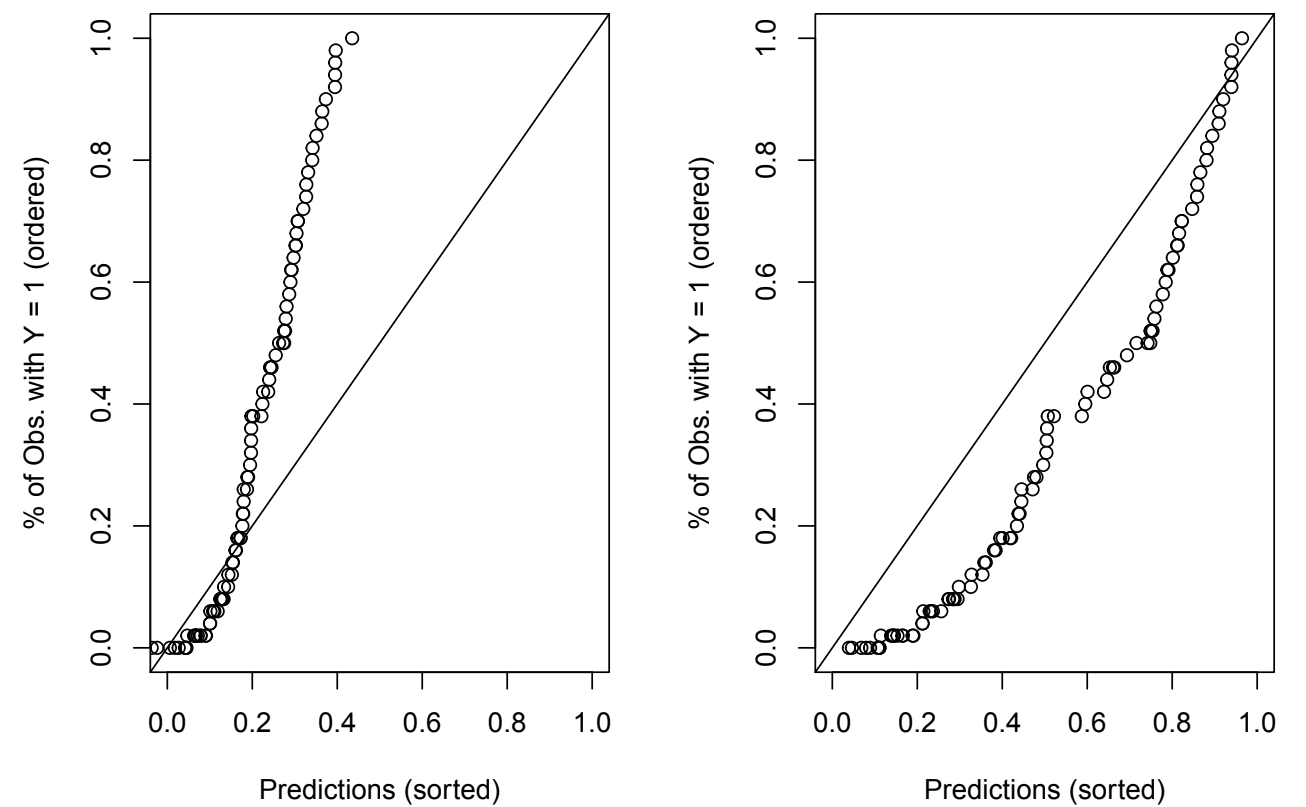
\includegraphics[width=0.8\textwidth]{figure_man/platts-scaling.png}
% \end{figure}

% \end{frame}


% \begin{frame}{Isotonic regression}

% \begin{itemize}
% \item The idea is to fit a piecewise-constant non-decreasing function instead of
% logistic regression with the pool adjacent violators algorithm
% ($\mathcal{O}(n)$).
% \item Basically, the algorithm goes through the data and looks for violations of
% the monotonicity constraint. If it finds one, it gets adjusted with the best
% possible fit under the constraint.
% \end{itemize}

% \begin{center}
% 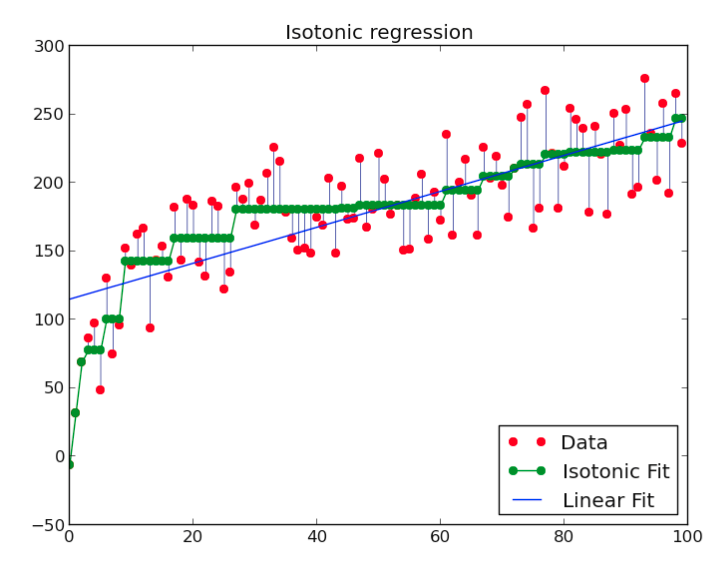
\includegraphics[width=0.5\textwidth]{figure_man/iso-reg.png}
% \end{center}
% \end{frame}
% \begin{frame}{Isotonic regression}

% \begin{figure}
% 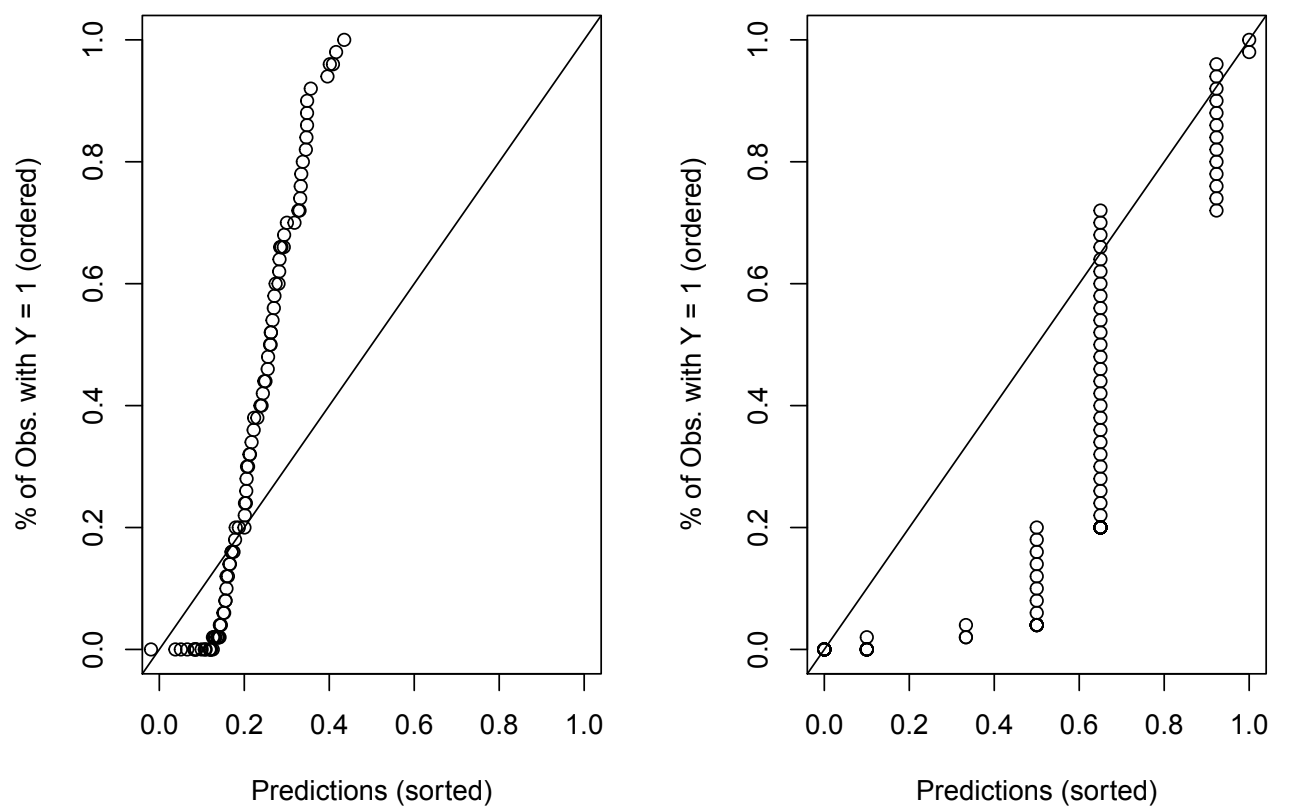
\includegraphics[width=0.8\textwidth]{figure_man/isotonic-reg.png}
% \end{figure}

% \end{frame}






% \begin{frame}{Diagnosis with Reliability Diagrams}
%     % https://www.cs.cornell.edu/~alexn/papers/calibration.icml05.crc.rev3.pdf
%     To Do: selbst coden
%     \begin{figure}
%         \centering
%         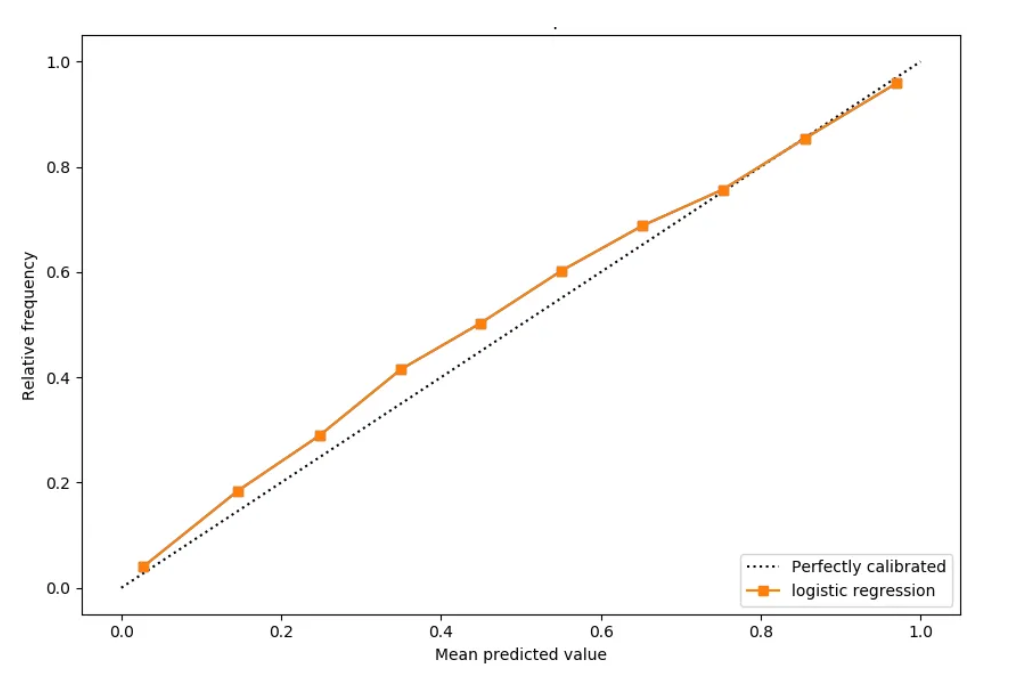
\includegraphics{figure/reliability_diagram.png}
%         % \caption{Caption}
%         % \label{fig:enter-label}
%     \end{figure}
% \end{frame}

% --------------------------------------

% \begin{frame}{Sources of Miscalibration}
% % https://classifier-calibration.github.io/assets/slides/clacal_tutorial_ecmlpkdd_2020_intro.pdf
% \begin{itemize}
%     \item Calibration is a characteristic of a learner, e.g., tree-based learners such as CART or random forests seldom produce probabilities close to 0 or 1 due to averaging class values. 
%     \item Miscalibration is related to accuracy: if the average class probability is higher or lower than accuracy, the model is said to be over- or underconfident.
%     \item \textbf{Underconfidence:} Probabilities are underestimating true incidences. This typically gives a sigmoidal reliability diagram.
%     $\Rightarrow$ We need to pull probabilities away from the center.
%     \item \textbf{Overconfidence:} Probabilities are overestimating true incidences.  This typically gives an inverse-sigmoidal reliability diagram. $\Rightarrow$ We need to push probabilities toward the center.
%     \item \textbf{Predicament:} Under- and overconfidence can coexist for different classes, requiring a simultaneous increase and decrease in different class probabilities.

% \end{itemize}
% \end{frame}

% \begin{frame}[t]
% 	\frametitle{Calibrating Probabilities}
% 	%\small
% 	\begin{itemize}
% % %		
% % 		\item Consider binary classification with a probabilistic score  classifier
% % %		
% % 		$$\fx = 2 \cdot \mathds{1}_{[ s(\xv) \ge c]} -1,$$
% % %		
% % 		leading to the prediction random variable $\yh = f(\xv).$ Let $\mathbf{S}=s(\xv)$ be the score random variable. 
% % %		
% % 		\item $f$ is calibrated iff $P(y=1~|~\mathbf{S}=s) = s$ for all $s\in [0,1].$
% %		
% 		\item Let $s(\xv)$ be the predicted (uncalibrated) score/probability of instance $\xv$ and $\mathbb{S}$ the set of possible scores produced by the classifier.
%         \item Different \emph{post-processing} methods have been proposed for the purpose of calibration, i.e., to construct a \emph{calibration function} 
% %		
% 		$$C: \, \mathbb{S} \to [0,1], $$
% 		such that $C(s(\xv))$ is well-calibrated.
		
% 		\item For learning a calibration function $C$, a set of \emph{calibration data} is used:
% 		$$
% 		\mathcal{D}_{cal} = \big\{ (s^{(1)}, y^{(1)}) , \ldots , (s^{(n)}, y^{(n)}) \big\} \subset \mathbb{S} \times \{ 0 , 1 \}
% 		$$ 
% 		\item This data should be different from the training data used to learn the scoring classifier. Otherwise, there is a risk of introducing a bias. 
		
% 	\end{itemize}
% \end{frame}

\begin{frame}[t]
  \frametitle{Calibrating Probabilities}

  \begin{itemize}
    \item Let $s(\xv)$ denote the predicted (uncalibrated) score for input $\xv$
    \item Define $\mathbb{S}$ as the set of possible scores produced by the classifier
    \item Goal: Construct a \emph{calibration function} $C$ that maps scores $s(\xv) \in \mathbb{S}$ to calibrated probabilities $C(s(\xv)) \in [0,1]$:
    \[
      C: \mathbb{S} \to [0, 1], \text{such that } C(s(\xv)) \approx P(y = 1 \mid s(\xv)) \text{ (well-calibrated)}
    \]
    \item To learn calibrator function $C$, use a separate \emph{calibration dataset}:
    \[
      \mathcal{D}_{\text{cal}} = \{ (s^{(i)}, y^{(i)}) \}_{i=1}^{n} \subset \mathbb{S} \times \{0, 1\}
    \]
    \item Important: $\mathcal{D}_{\text{cal}}$ must be disjoint from the training data used to learn the scoring classifier to avoid bias in estimated calibration
  \end{itemize}

\end{frame}


\begin{frame}[t]
	\frametitle{Empirical binning}
	% https://link.springer.com/article/10.1007/s10994-023-06336-7
\emph{Empirical binning} partitions predicted scores \( s \in \mathbb{S}\) into bins \( B_1, \ldots, B_M \) and defines a (piecewise constant) calibration function \( C \) by:

\[ 
C(s) = \bar{p}_{J(s)} = \frac{\sum_{i=1}^n \mathds{1}[ s^{(i)}  \in B_{J(s)}] \cdot y^{(i)}}{|B_{J(s)}|}, \, \text{ where }
\]

\begin{itemize}
    \item \( J(s) \in \{1, \dots, M\}\) is the bin index that \( s \) belongs to (i.e., \( s \in B_{J(s)} \))
    \item \( s^{(i)} = s(\xi) \) is the score  and \( y^{(i)} \) the label of instance \( i \) % (with \( y^{(i)} = 1 \) indicating a positive instance)%,
%- \( |B_{J(s)}| \) is the number of instances in the bin \( B_{J(s)} \).
    \item numerator counts the number of positive instances within \( B_{J(s)} \)
%- \( |B_{J(s)}| \) counts the total number of instances within the bin \( B_{J(s)} \).
\end{itemize}

\( \Rightarrow C \) maps \( s \) to \( \bar{p}_{J(s)} \) (average proportion of positive instances in \( B_{J(s)} \))  %\( \bar{p}_{J(s)} \) represents the average proportion of positive instances in the bin \( B_{J(s)} \), and \( C(s) \) is the calibration function that maps the score \( s \) to this average proportion.

  \vfill
  \centering
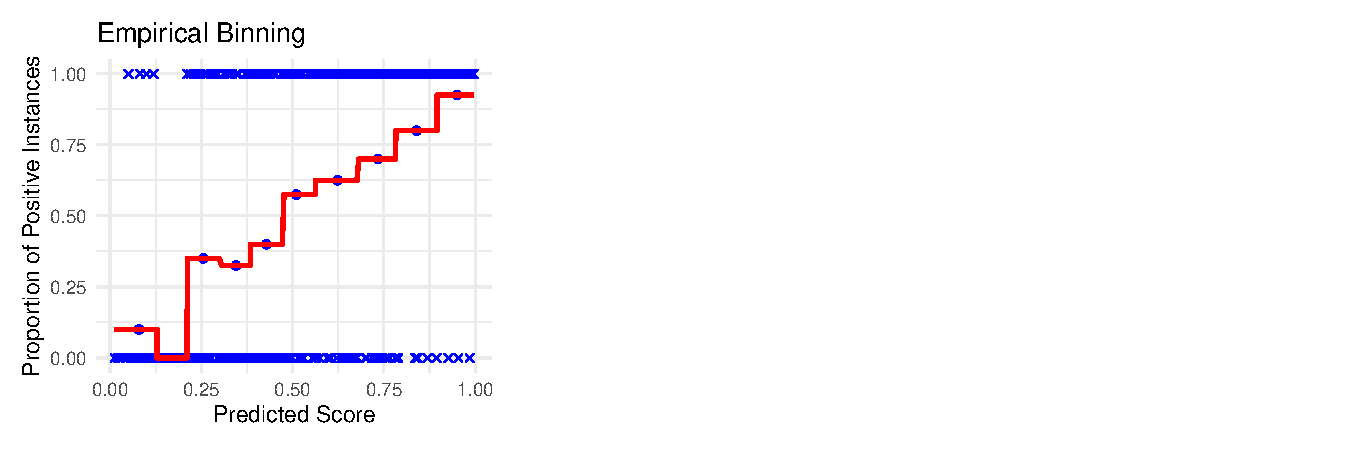
\includegraphics[width=0.8\textwidth]{figure/calibration_methods1.pdf}
\end{frame}




\begin{frame}[t]
	\frametitle{Platt scaling
    % OLD
%\citebutton{Niculescu-Mizil et al., 2005}{https://www.cs.cornell.edu/~alexn/papers/calibration.icml05.crc.rev3.pdf}
% NEW
\furtherreading{MIZIL2005} }

    %TODO requires: unbounded outputs before sigmoid/ softmax, good for Neuronal Networks, SVM, boosted trees
    %TODO reference Alexandru Niculescu-Mizil and Rich Caruana. “Predicting Good Probabilities with Supervised Learning.” In Proceedings of the 22nd International Conference on Machine Learning (ICML), 2005.
	
\emph{Platt scaling} applies logistic regression to predicted scores $s \in \mathbb{S}$, i.e., it fits a calibration function $C$ minimizing the log-loss on $\mathcal{D}_{cal}$ by:
		$$
		C(s) = \frac{1}{1 + \exp( \theta_0 + \theta_1 \cdot s) } , \, \text{ where }
		$$

  \begin{itemize}
    \item $\theta_0$ is the intercept, and $\theta_1$ the slope estimated by the logistic regression
    \item Requires: unbounded outputs before sigmoid/softmax, good for Neural Networks, SVM, boosted trees
\end{itemize}
  \vfill\centering
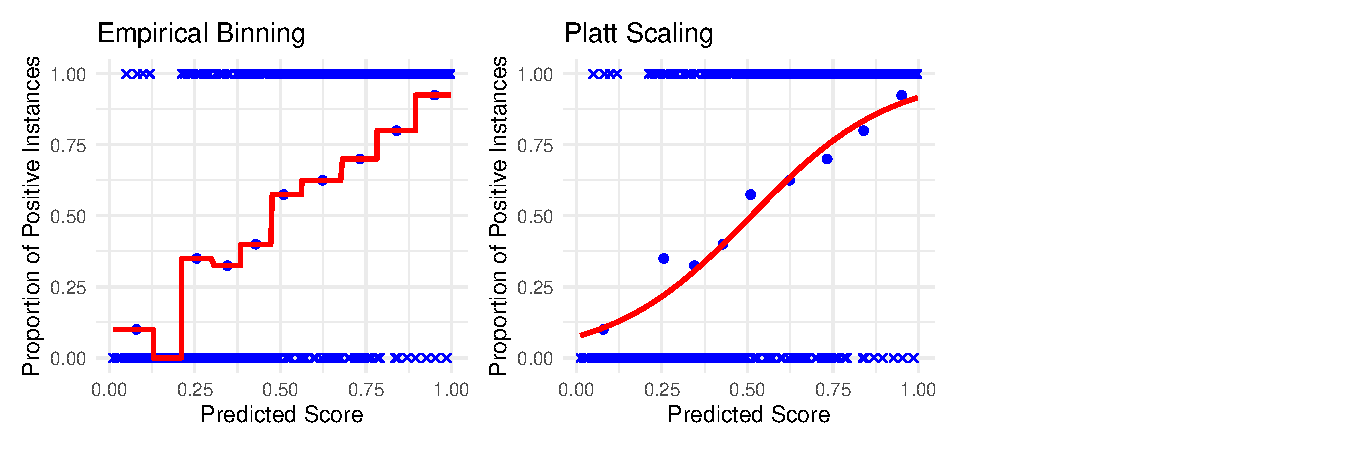
\includegraphics[width=0.8\textwidth]{figure/calibration_methods2.pdf}
\end{frame}


\begin{frame}[t]
	\frametitle{Isotonic regression % OLD
%\citebutton{Kull et al., 2017 }{http://proceedings.mlr.press/v54/kull17a/kull17a.pdf}
% NEW
\furtherreading{KULL2017}}
    
    %TODO requires bounded or monotonic relationship with probabilities
    %TODO reference http://proceedings.mlr.press/v54/kull17a/kull17a.pdf
	
	\begin{itemize}
		%\item The sigmoidal transformation fit by Platt scaling is appropriate for some methods (e.g., support vector machines) but not for others. 
		\item \emph{Isotonic regression} combines the non-parametric character of empirical binning with the monotonicity guarantee of Platt scaling by minimizing
		$$
		\sum_{i=1}^n w_i \, (C(s^{(i)}) - y^{(i)})^2 
		$$
		subject to the constraint that $C$ is isotonic: $C(s) \leq C(t)$ for $s <t$. 
		\item 
		Note: $C$ is evaluated only at a finite number of points; in-between, one may (linearly) interpolate or assume a piecewise constant function. 
		
	\end{itemize}
 \vfill\centering
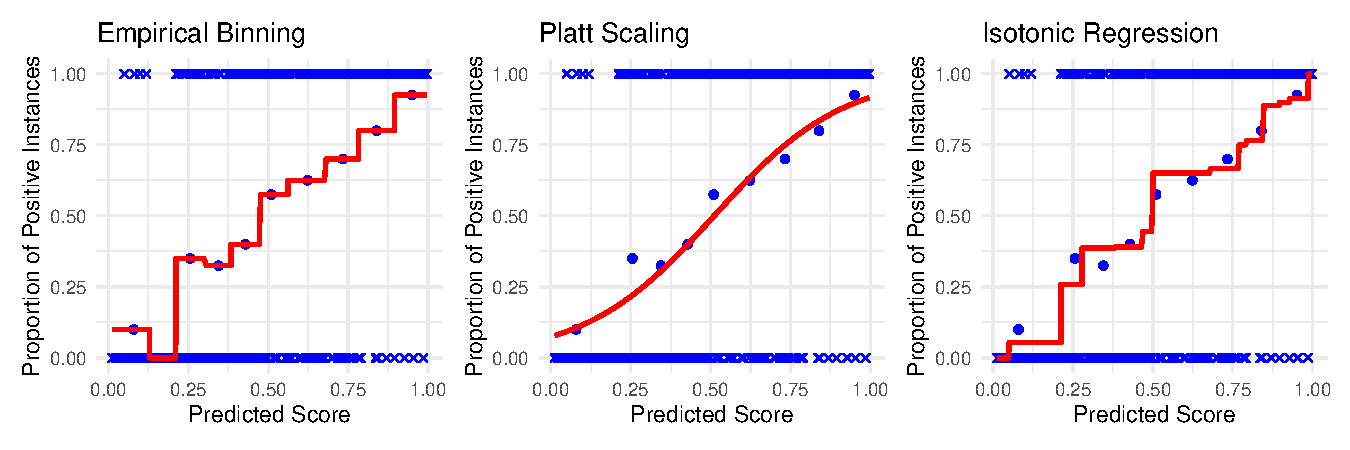
\includegraphics[width=0.8\textwidth]{figure/calibration_methods3.pdf}
\end{frame}



\begin{frame}[t]
	\frametitle{Isotonic Regression - PAVA}
	
	\begin{itemize}
        \item Optimization can be solved by the pool-adjacent violators algorithm (PAVA) by sorting scores such that
		$$
		s^{(1)} < s^{(2)} < \ldots < s^{(n)}\, .
		$$
		% We then seek values $c_1 \leq c_2 \leq \ldots \leq c_n$ which minimize
		% $$
		% \sum_{i=1}^n w_i ( c_i - y^{(i)})^2 \, .
		% $$
		\item Initialize bins $B_i$ for each observation $(s^{(i)} , y^{(i)})$
        \item Assign to all scores $s \in B_i$: $C(s) = y^{(i)}$ with initial width $w(B_i) = 1$.
		
		\item A merge operation combines two adjacent bins $B_j$ and $B_k$ into a new bin $B = B_j \cup B_k$ with width $w(B) = w(B_j) + w(B_k)$ and 
		$$
		C(B) = \frac{w(B_j) C(B_j) + w(B_k) C(B_k)}{w(B_j) + w(B_k)} \, .
		$$
		
		
\item The algorithm looks for violations of the monotonicity constraint and adjusts them with the best possible fit under the constraint ($\mathcal{O}(n)$).
	\end{itemize}
\end{frame}

\begin{frame}[t]
	\frametitle{Isotonic Regression - PAVA}
	 PAVA iterates the following steps (simplified to avoid notational overload):

		\begin{itemize}
        \setlength\itemsep{0pt} % or 0pt
			\item[(1)]<1-> Find first violating adjacent bins $B_i$ and $B_{i+1}$ such that $C(B_i) > C(B_{i+1})$.
			\item[(2)]<1-> Merge $B_i$ and $B_{i+1}$ into a new bin $B$. Stop if no violation occurred.
			\item[(3)]<2-> If $C(B) < C(B_{i-1})$ for the left neighbor bin $B_{i-1}$, merge also these bins and continue until no more violations are found (monotonicity).
			\item[(4)]<2-> Continue with \textbf{(1)}.
		\end{itemize}
	
	\begin{center}
	\includegraphics<1>[width=0.6\textwidth, trim=0px 200px 0px 0px, clip]{figure/pic-pava}
        \includegraphics<2->[width=0.6\textwidth, trim=0px 0px 0px 0px, clip]{figure/pic-pava}
	\end{center}
\end{frame}

% \begin{frame}[t]
% 	\frametitle{Isotonic Regression - PAVA}
	
% 	\begin{itemize}
% 		\item Note that, in the case of binary classification, the target values $y^{(n)}$ are all in $\{ 0, 1 \}$:
% 	\end{itemize}
	
% 	\medskip 
	
% 	\begin{center}
% 		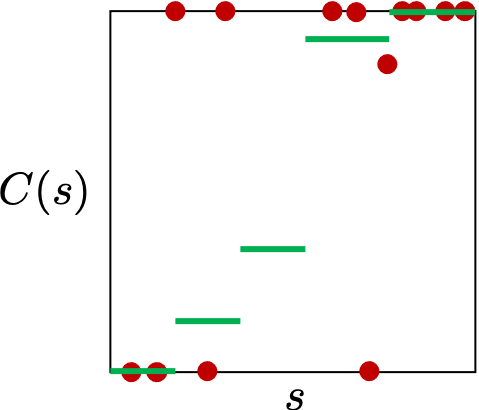
\includegraphics[width=0.4\textwidth]{figure/pic-pava2}
		
% 	\end{center}
% \end{frame}


% \begin{frame}[t]
% 	\frametitle{Outlook: Multi-class calibration}
	
% 	\begin{itemize}
%         \itemsep1em
% 		\item Calibration methods also exist for the multi-class case (i.e., classification problems with more than two classes).
% 		\item Then, however, the problem becomes conceptually more difficult (and is still a topic of ongoing research).
% 		\item 
% 		While essentially coinciding for binary classification, the following definitions of calibration (leading to increasingly difficult problems) can be distinguished for more than two classes:
% 		\begin{itemize}
% 			\item Calibration of the highest predicted probability (confidence calibration) 
% 			\item Calibration of the marginal probabilities (class-wise calibration)
% 			\item Calibration of the entire vector of predicted probabilities (multi-class calibration)
% 		\end{itemize}
%         \item Recently, native multi-class calibration methods extended Platt scaling by adding a calibration layer between the logits of the neural network and the softmax layer. 
% 	\end{itemize}
% \end{frame}


%TODO add workflow here

%Split data in train, calibrate test
%After training, find best calibration method by evaluating on calibrate

%add reference on workflow: http://proceedings.mlr.press/v54/kull17a/kull17a.pdf

%Tuning prior calibration leads to better results than tuning the calibrated learner
%CV calibration leads to better results than holdout calibration




\begin{frame}{How to Split Data for Calibration?  \furtherreading{ESKANDAR2023}}% OLD
%\citebutton{Eskandar, 2023}{https://medium.com/@eskandar.sahel/applying-calibration-techniques-to-improve-probabilistic-predictions-in-machine-learning-models-c175c2e38ffc}


\textbf{Problem:} How to avoid overfitting the calibrator during training?

\vspace{0.5em}
\textbf{Deployment scenario:} 
\begin{itemize}
  \item Inducer (ML algorithm \& hyperparameters) already selected
  \item Want to calibrate predictions of resulting model using all available data
\end{itemize}
\pause

\vspace{0.5em}
\textbf{Naive solution:} Use hold-out calibration set

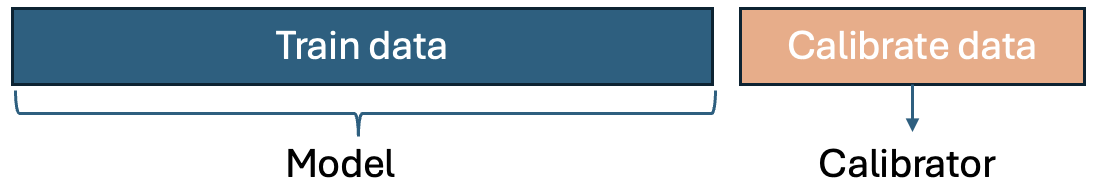
\includegraphics[width=\linewidth]{figure_man/CalibWorkflow1.png}

\vspace{0.5em}
\textbf{Limitation:} Does not utilize full dataset for training model and calibrator

\vspace{0.5em}
\visible{\textbf{Idea:} Use $k$-fold CV to use available data more efficiently}
\end{frame}


\begin{frame}{CV for Calibration: Per-Fold Strategy}
%\textbf{Per-fold strategy:}
\begin{itemize}
  \item Fit model and calibrator on each CV fold separately
  \item Use fold-wise models to generate (uncalibrated) predictions and fold-wise calibrators to calibrate them
  \item Average fold-wise calibrated predictions
\end{itemize}

{\centering
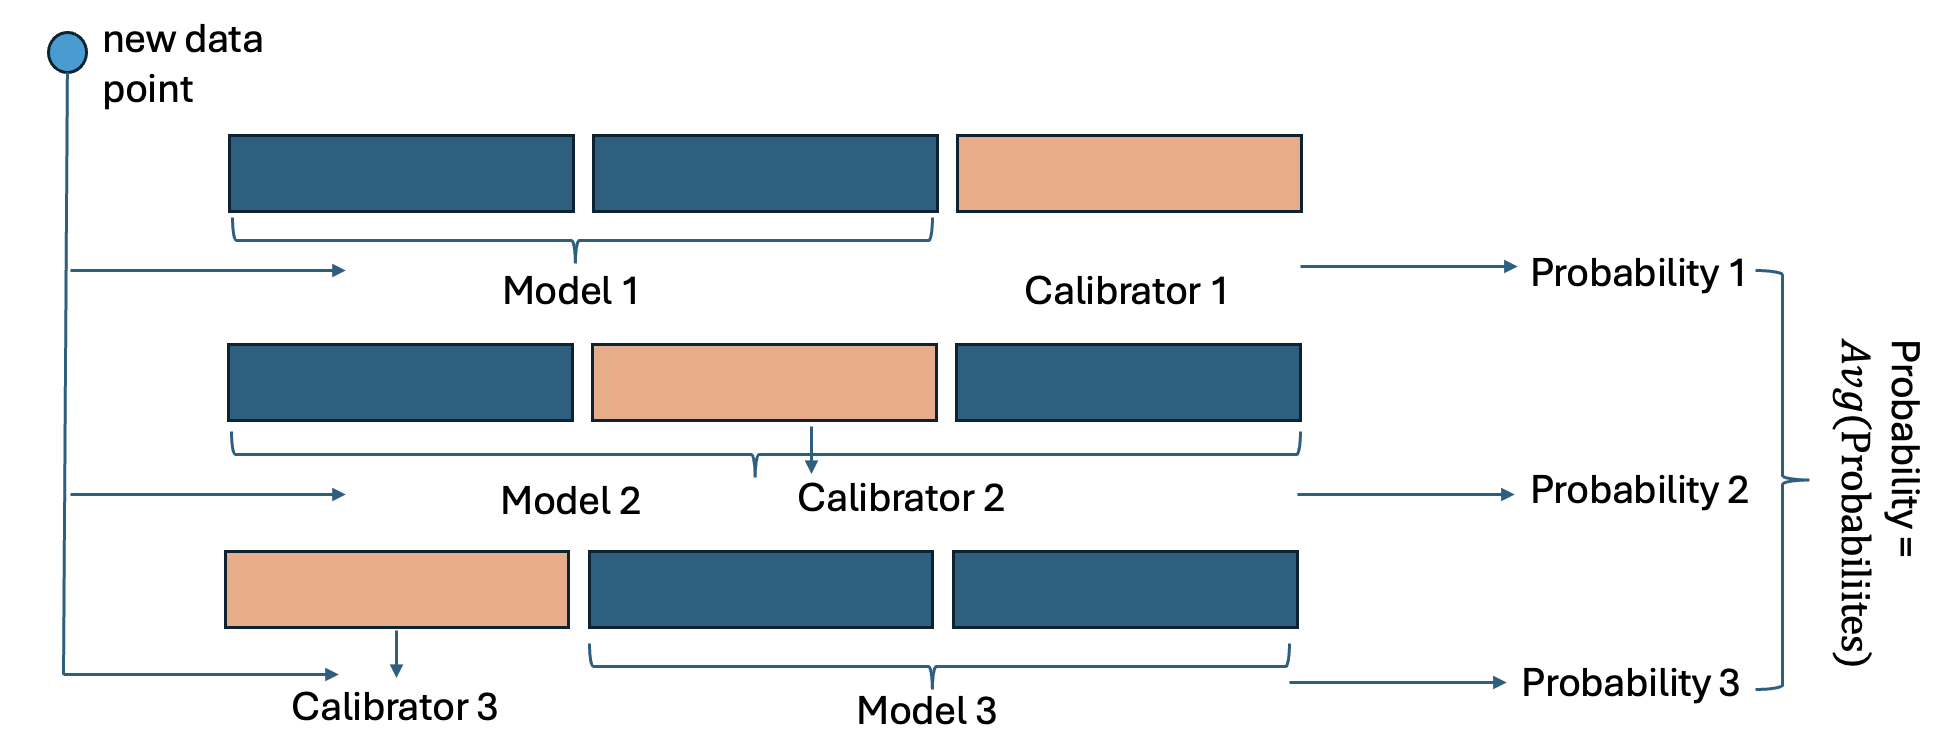
\includegraphics[width=0.9\linewidth]{figure_man/CalibWorkflow2.png}}

\pause

\textbf{Drawback:} Computationally inefficient (requires training $k$ models and $k$ calibrators); none are trained on full data $\Rightarrow$ pessimistic bias in calibration.

\visible{\textbf{Alternative:} CV with pooled out-of-fold (OOF) predictions}
\end{frame}


\begin{frame}{CV for Calibration: Pooled OOF Strategy}
%\textbf{Steps:}
\begin{enumerate}
  \item Fit final model on entire dataset
  \item Perform CV and generate out-of-fold predictions from CV models
  \item Train calibrator on pooled OOF CV predictions (uses all observations)
  \item Deploy: predict with final model, calibrate with pooled calibrator\\
  \item[$\Rightarrow$] \textbf{Advantage:} One final model + one calibrator, both trained on all data
\end{enumerate}

\vspace{1em}
\centering
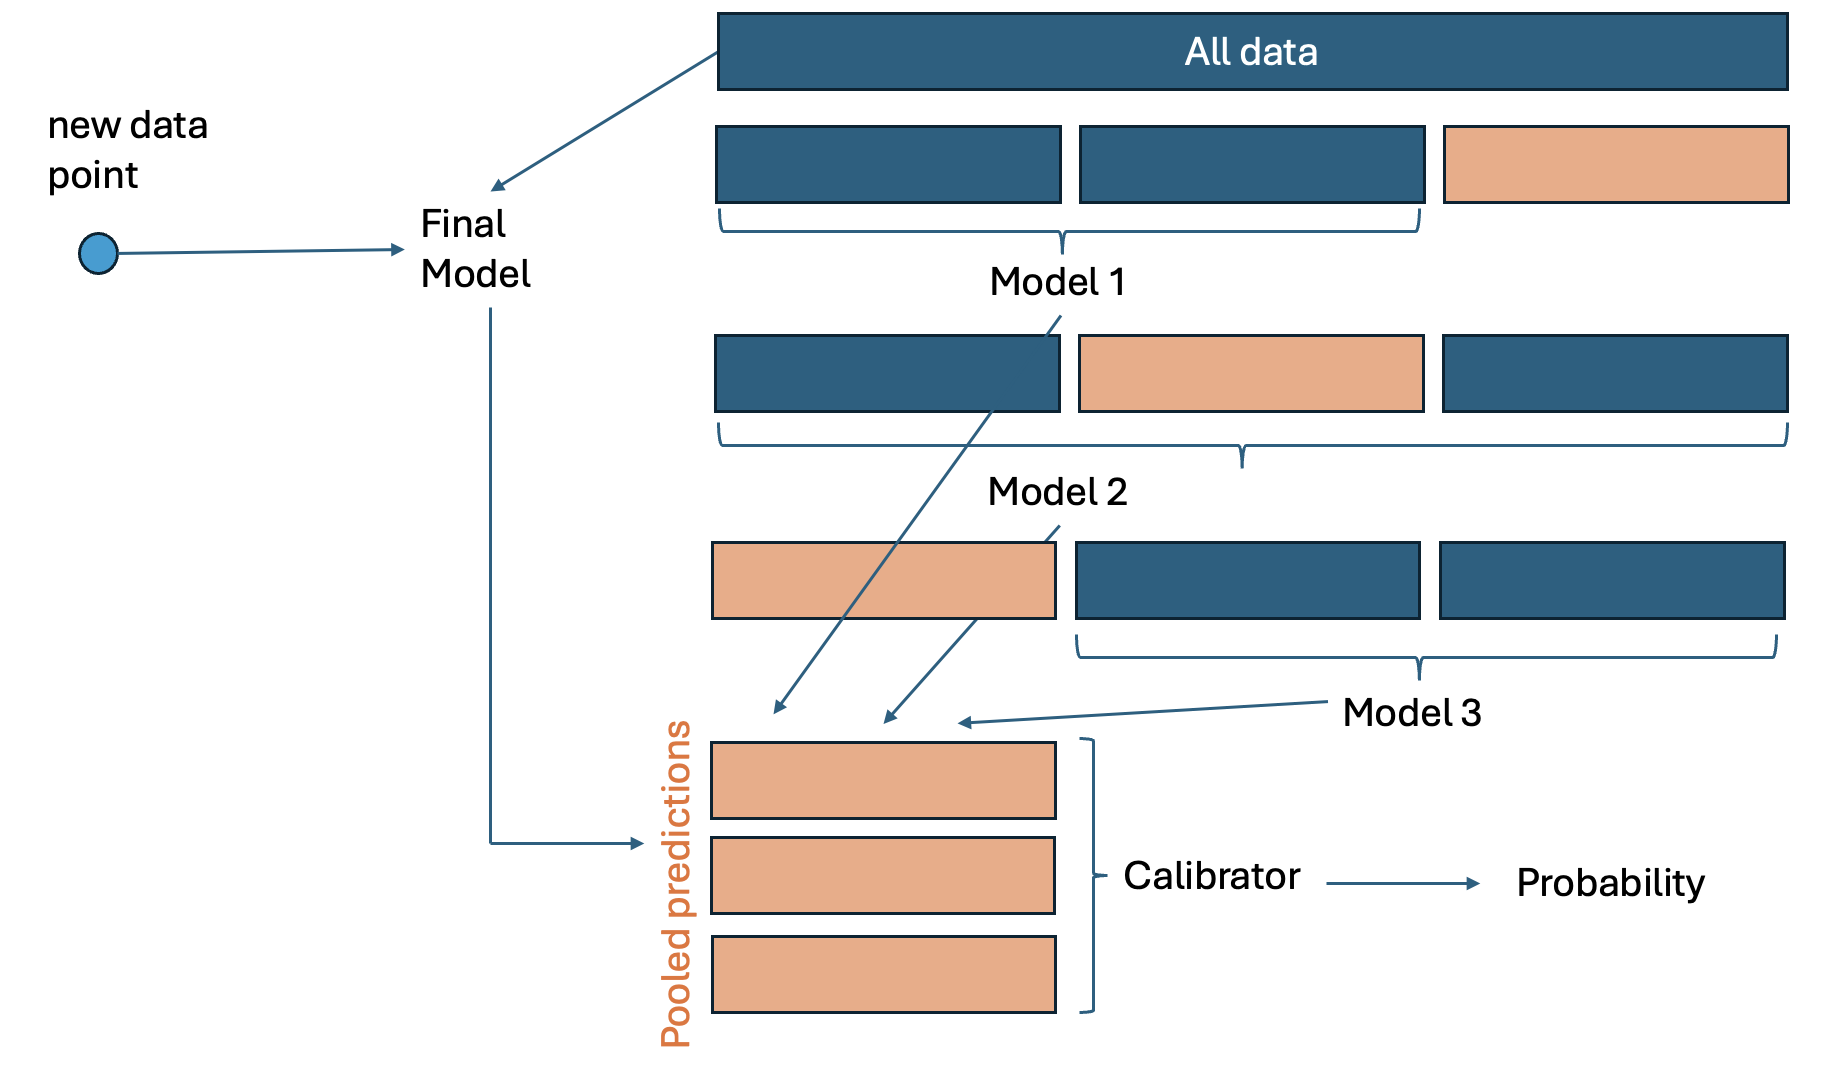
\includegraphics[width=0.75\linewidth]{figure_man/CalibWorkflow3.png}

\end{frame}


\begin{frame}{When Evaluation is Needed}
\textbf{Setting:} When the aim is to tune hyperparameters or estimate performance, we require an independent test set (besides the train and calibration set).
%Performance metrics or hyperparameter tuning required

\vspace{0.5em}
\textbf{Option 1:} Simple hold-out split (train set, calibration set, test set)

\vspace{0.5em}
\textbf{Option 2:} Nested Cross-Validation
\begin{itemize}
  \item Inner loop: Train model \& calibrator (per-fold or pooled OOF strategy) 
  \item Outer loop: Evaluate generalization performance
\end{itemize}

\centering
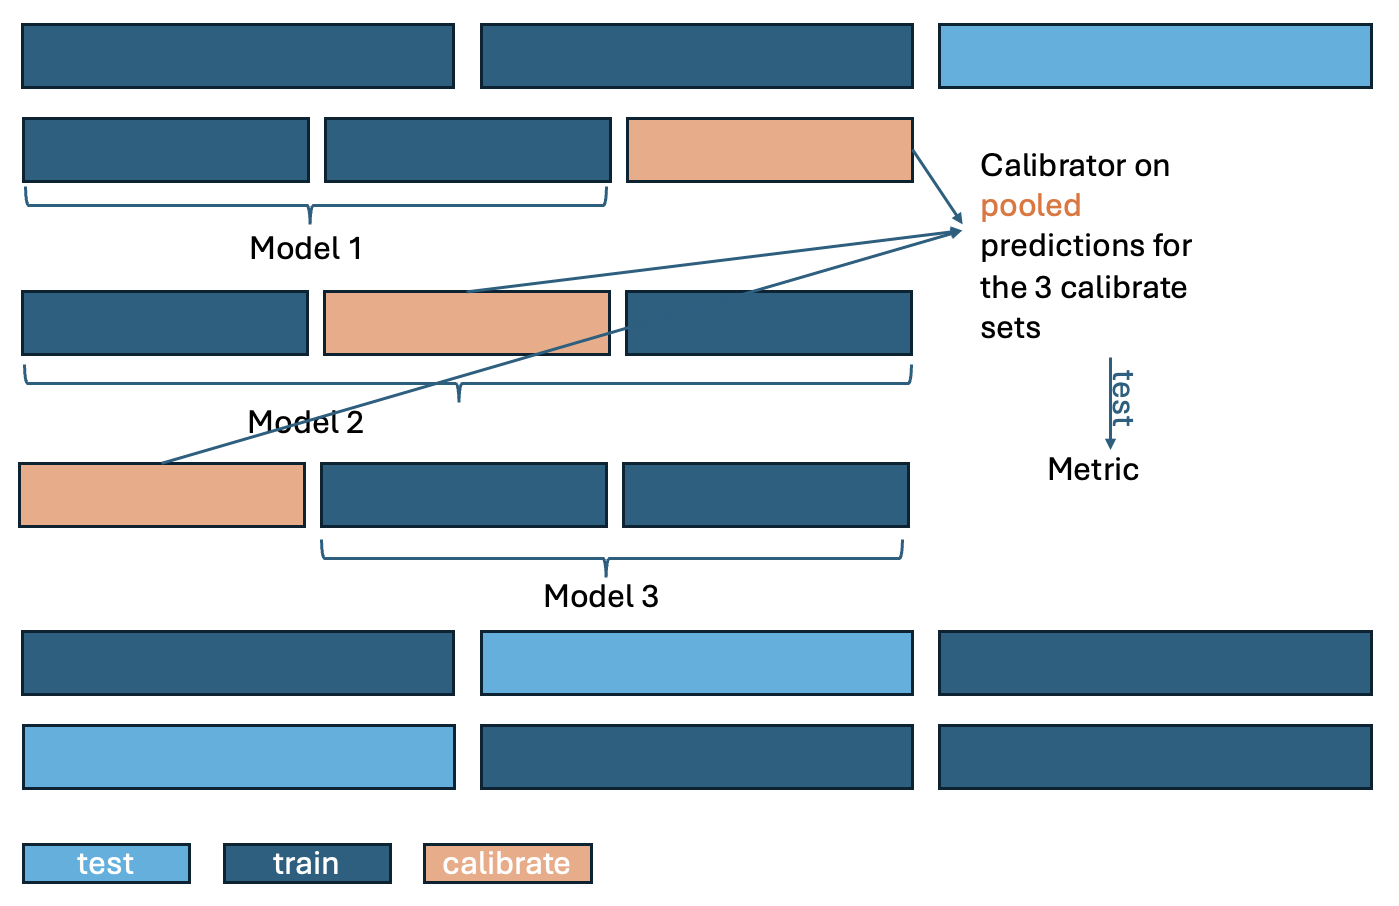
\includegraphics[width=0.6\linewidth]{figure_man/CalibrationCVPooled.png}
\end{frame}

% \begin{frame}{Calibration Workflow % OLD
%\citebutton{Eskandar, 2023}{https://medium.com/@eskandar.sahel/applying-calibration-techniques-to-improve-probabilistic-predictions-in-machine-learning-models-c175c2e38ffc}
% NEW
% \furtherreading{Eskandar2023}}

% \textbf{Question}: How to split the data for training the model and training the calibrator, so that we don't overfit the calibrator?

% \textbf{Given Situation}: We have already settled on a specific inducer and now want to train the model and calibrator on all our data for deployment.

% \textbf{Simplest Solution}: Hold out split.

% 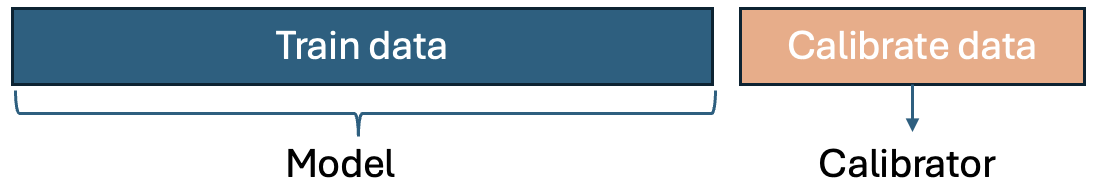
\includegraphics[width = \linewidth]{figure_man/CalibWorkflow1.png}

% \textbf{But}: We want to use ALL the data for training the model and calibrator \\ $\Rightarrow$ \textbf{Cross-validation}

% \begin{itemize}
%     \item CV per fold
%     \item Pooled CV
% \end{itemize}

% \end{frame}


% \begin{frame}{Calibration Workflow}
% \textbf{Option A}: Cross-validation per fold
% 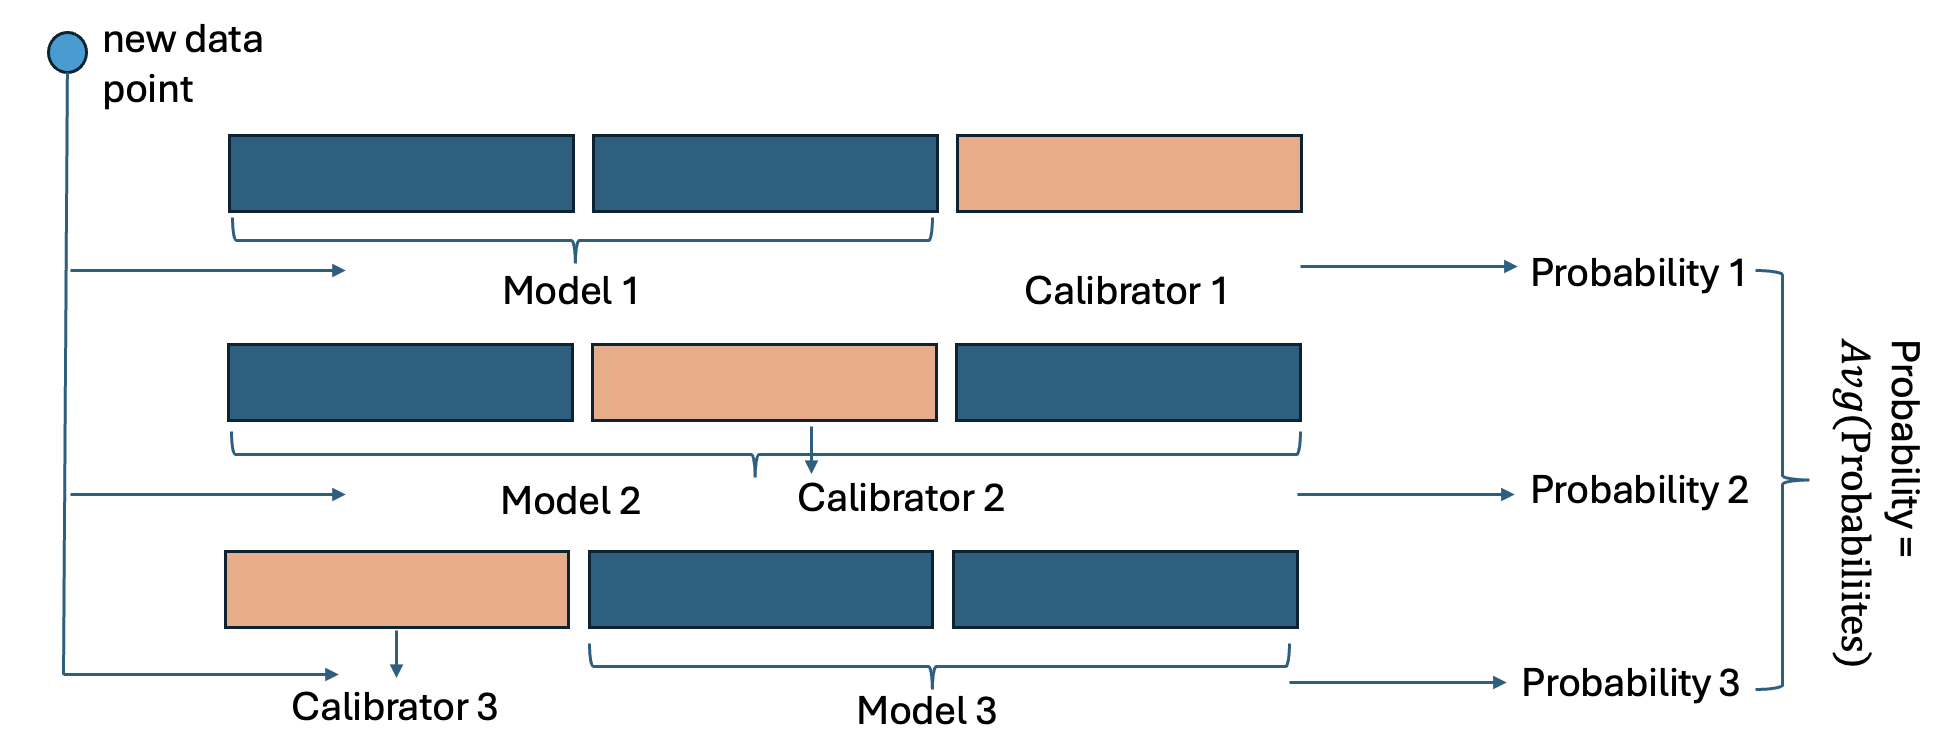
\includegraphics[width = \linewidth]{figure_man/CalibWorkflow2.png}

% Disadvantage:
% \begin{itemize}
%     \item we fit multiple models and calibrators, which takes a long time
%     \item none of the calibrators is fitted on all data
% \end{itemize}

% $\Rightarrow$ Pooled CV
% \end{frame}

% \begin{frame}{Calibration Workflow}
% \textbf{Option B}: Cross-validation pooled
% 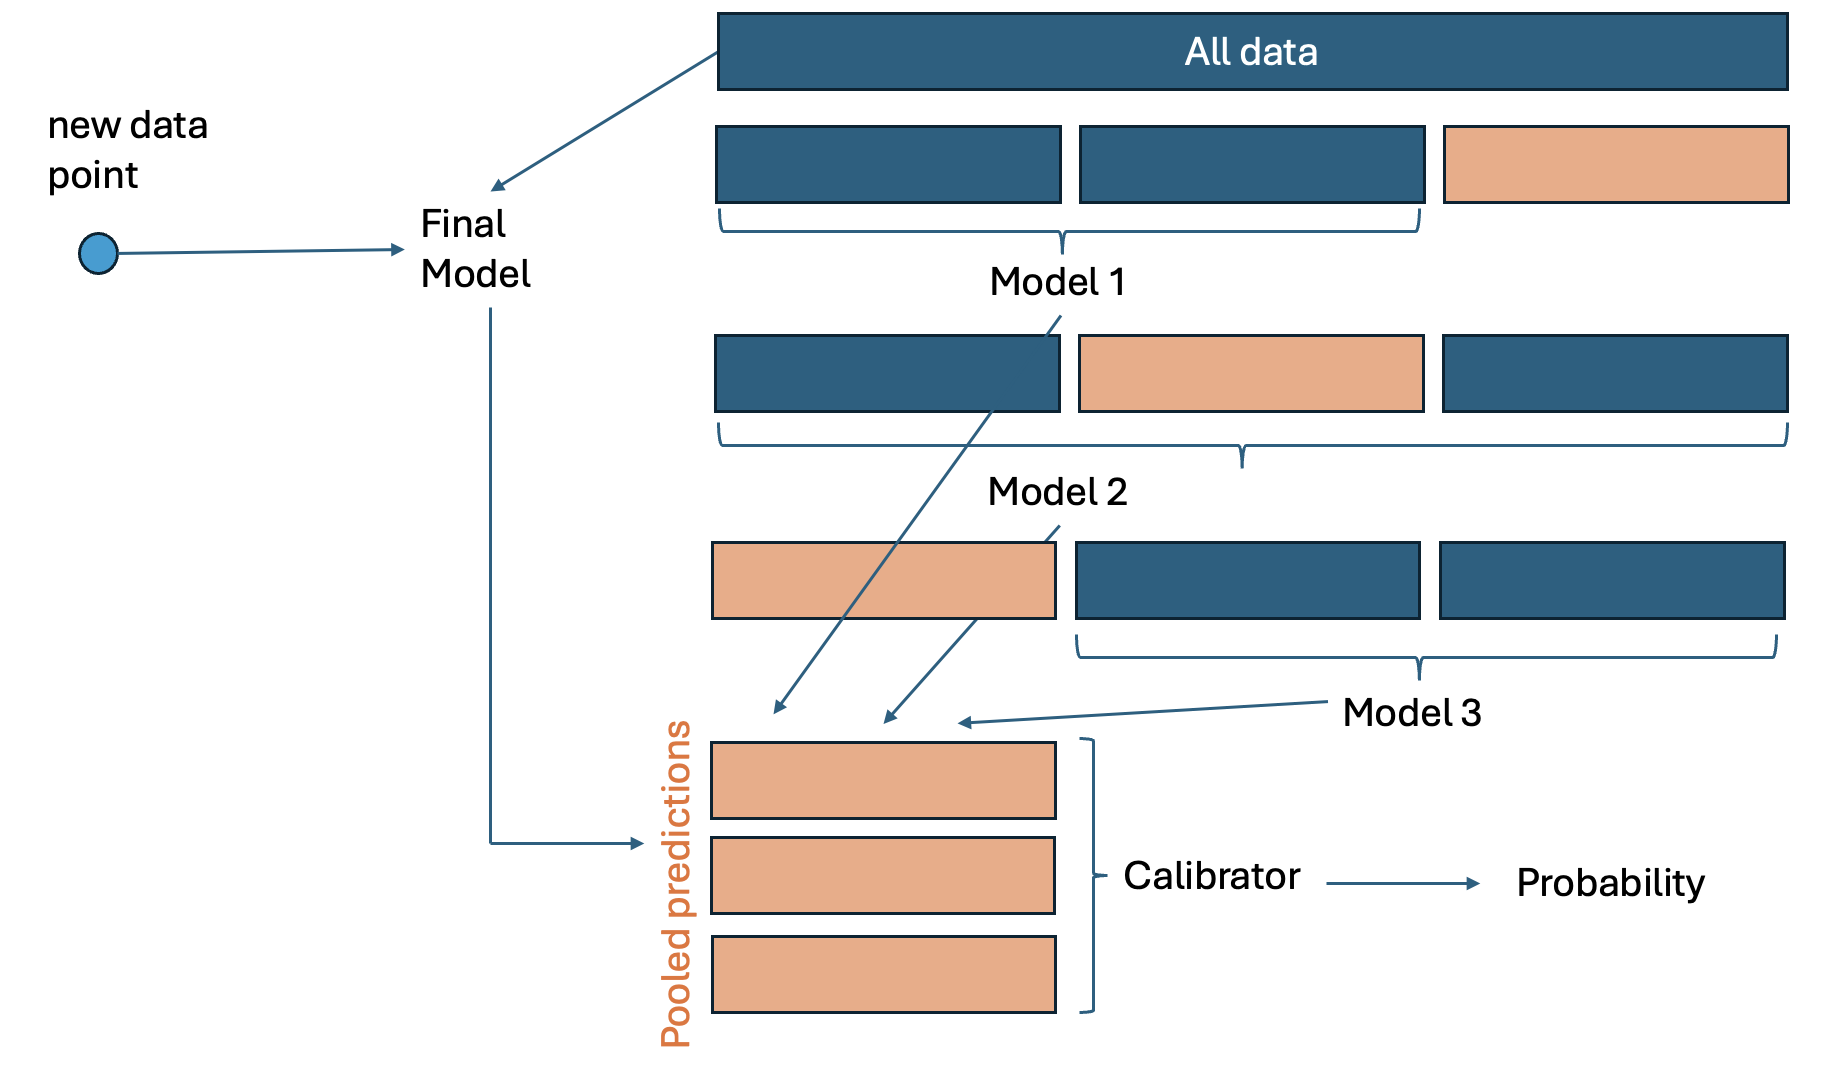
\includegraphics[width = 0.7 \linewidth]{figure_man/CalibWorkflow3.png}
% \begin{itemize}
%     \item Fit final model on all data
%     \item Fit multiple models on CV folds
%     \item Fit calibrator using pooled out-of-fold predictions (uses all observations) %and data
%     \item Pass new data point through final model and calibrator\\
%     $\rightarrow$ Only one model and calibrator, fitted on all data
% \end{itemize}
% \end{frame}

% \begin{frame}{Calibration Workflow}

% \textbf{Question}: How to split the data for training the model and training the calibrator, so that we don't overfit the calibrator?

% \textbf{New Situation}: We want to tune or compute performance metrics, i.e. we also need untouched test data.

% \textbf{Solution}:
% \begin{itemize}
%     \item Simple: Hold-out-split in train, calibrate and test (three sets)
%     \item Better: Nested Cross-validation, i.e. per-fold:
% \end{itemize}

% 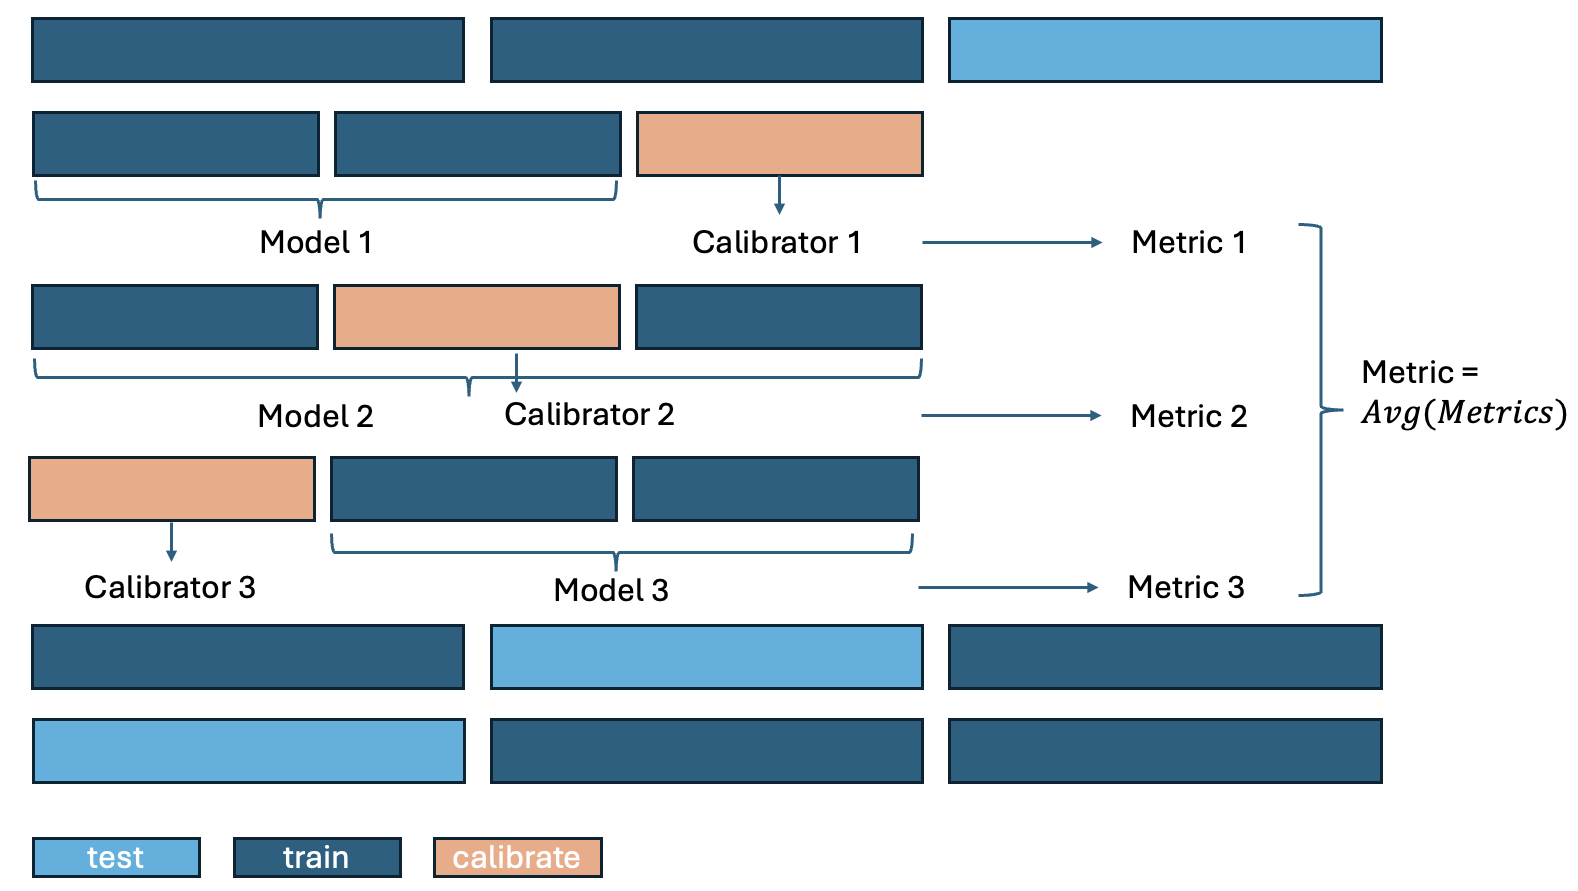
\includegraphics[width = 0.7 \linewidth]{figure_man/CalibrationCVFold.png}
    
% \end{frame}

%reference for calibration data split:
%- https://onlinelibrary.wiley.com/doi/full/10.1002/sim.9921 2 sets hold out
%- http://proceedings.mlr.press/v70/guo17a/guo17a.pdf 3 sets hold out
%- https://medium.com/@eskandar.sahel/applying-calibration-techniques-to-improve-probabilistic-predictions-in-machine-learning-models-c175c2e38ffc 5 fold cross validation




\begin{frame}{Example: Calibration Plot (Revisited)}
%Draw some conlusion in text form (i.e. all calibrations improved the original SVC)


Calibrating a SVC with Platt's scaling and isotonic regression:
\begin{center}
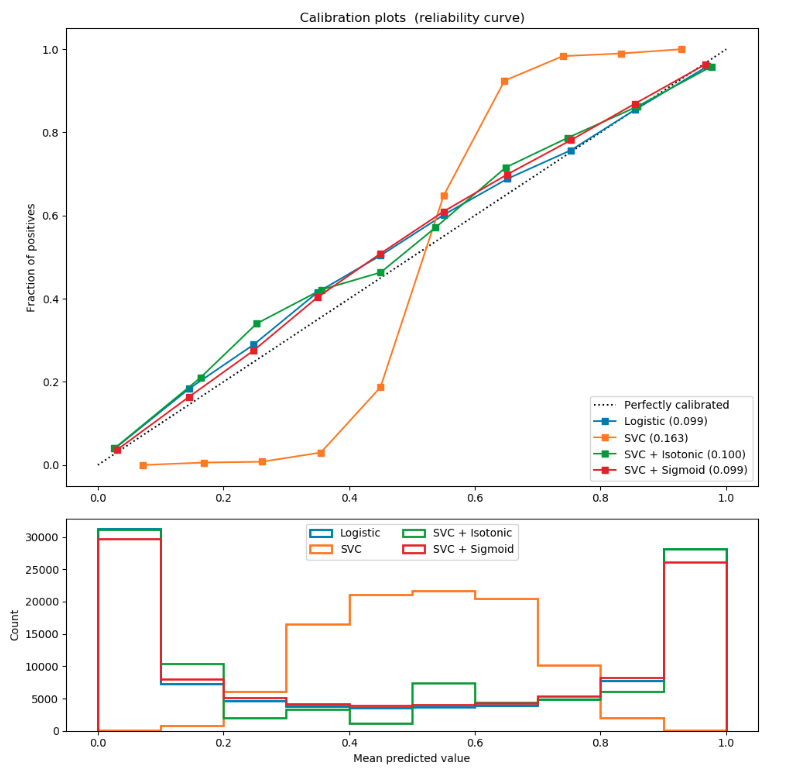
\includegraphics[width=0.5\textwidth]{figure_man/calibration2.png}
\end{center}
$\Rightarrow$ all calibrations improved the original SVC

\end{frame}

\begin{frame}{Summary: Why Is Calibration Important?}

    \begin{itemize}
        \item \textbf{Interpreting Predicted Probabilities:}
            \begin{itemize}
                %\item They should accurately reflect actual risks or frequencies of events.
                \item Good calibration ensures that predicted probabilities %match observed frequencies to 
                accurately reflect actual risks or frequencies of events.
                \item[$\Rightarrow$] Otherwise, predictions are just scores that happen to lie in $[0,1]$.
            \end{itemize}
        \item Instance-based probability evaluation metrics, such as Brier score or log-loss, always measure calibration (plus something else).
        \item \textbf{Example: Medical Diagnosis}
            \begin{itemize}
                \item Poor calibration: Only half of patients with 90\% predicted probability of a disease actually have it.
                \item Good calibration: 90\% of patients with 90\% predicted probability of a disease actually have it.
            \end{itemize}
    \end{itemize}
\end{frame}

\endlecture
\end{document}
